\section{A lexical sample}\label{a-lexical-sample}

To observe some of these high level institutions, I draw sets of
journals from four social science disciplines--anthropology, sociology,
economics, and political science--and I draw these in blocks from the
same publisher. Journals were selected from the disciplinary
affiliations signaled in their titles. From a JSTOR master list of
archived materials, journals were selected if they contained any of the
disciplinary prefixes anth-, soci-, econ-, and poli-. \{\{Though not all
journals that are affiliated with a discipline signal this with a word
containing the signature prefix, those that do are affiliated with a
high degree of accuracy. Soci is an exception, and journals like the
Royal Society of Statistics {[}madeup{]} are excluded.\}\} This list was
cross referenced with the TR WOK database.

Following these trends in the use of prefixes, we develop a sample or
journals that use them under the assumption that these signal domain
relevance for the disciplines.

We reduce the sampling frame in several steps. First, we require that
the journal publisher be located in the United States. Second, we
require that the journal be included in the JSTOR database. Third, we
require that the journal title contain, with some exceptions, at least
one of the prefixes . Of the journals in the WOK master list, these
criteria limit the sample to titles or less than half of a percent of
the original sampling frame.

The WOK master as of listed titles. It is not clear what sample of
historical population of journals this represents, but it is a
substantial substantive starting point.

The source data are observations on documents spanning years.

Each study depends on a database of records of the contents of journals.
This database is compiled from two sources, JSTOR and the Thompson
Reuters Web of Knowledge Social Science Citation Index (WOK).

\section{Sources}\label{sources}

\subsection{Google Books}\label{google-books}

\subsection{Thompson Reuters Web of
Knowledge}\label{thompson-reuters-web-of-knowledge}

\subsection{JSTOR Data for Research}\label{jstor-data-for-research}

\section{Research Databases}\label{research-databases}

\subsection{Sample Selection}\label{sample-selection}

\subsection{Entity Recognition}\label{entity-recognition}

\subsection{Formats}\label{formats}

\subsubsection{Edgelist}\label{edgelist}

\begin{figure}[htbp]
\centering
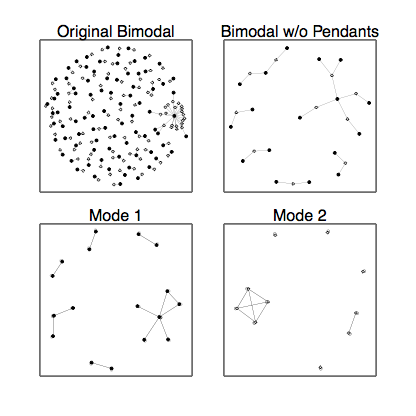
\includegraphics{~/prd/tex/fig/h-2modes.png}
\caption{Mode Projections}
\end{figure}

\subsubsection{Flat + k-Clique}\label{flat-k-clique}

\subsubsection{Survival}\label{survival}

\section{Drawer}\label{drawer}
